\chapter{Metode og proces}

I dette kapitel er der beskrevet kort hvilken analyse- og designmetode der er anvendt i bachelorprojektet. 

\section{Analyse og designmetode}

Dette afsnit har til formål at beskrive hvilke tekniske metoder, der er benyttet af udarbejdelsen af bachelorprojektet. Primært er der tale om metoder fra faget ISE. I dette afsnit bliver der også beskrevet hvilke arbejdsredskaber, der er benyttet til udførelse af bachelorprojektet og rapporten.\\

Udviklingsforløbet er udarbejdet efter V-modellen, figur \ref{fig:vmodel} og ASE-modellen figur \ref{fig:asemodel} \cite{IngeniorhojskolenAarhusUniversiteta}, som er udviklet af Aarhus Ingeniørskole. ASE-modellen anvendes til udvikling af software og hardware, som er delt op i faser. For hver fase kommer en række artefakter som tilsammen resulterer i et veldokumenteret bachelorprojekt. Disse faser kombineres med V-modellen. I dette bachelorprojekt er der udført modultest på alle moduller opført i både hardware og software. Efter at kunne godkende modultestene, er en integrationstest blevet udført, hvor det bygget hardware og software er sammensat og testet som et samlet system. Her gøres det klart at systemet fungerer som intentionen, inden accepttesten nåes. Accepttesten undersøger om alle krav specificeret i kravspecifikationen er overholdt. Vejleder, Thomas Nielsen, Adjunkt på Institut for Ingeniørvidenskab på Aarhus Universitet, har deltaget i udførelsen af accepttesten, godkendt og underskrevet den. 

\begin{figure}[H]
\centering
{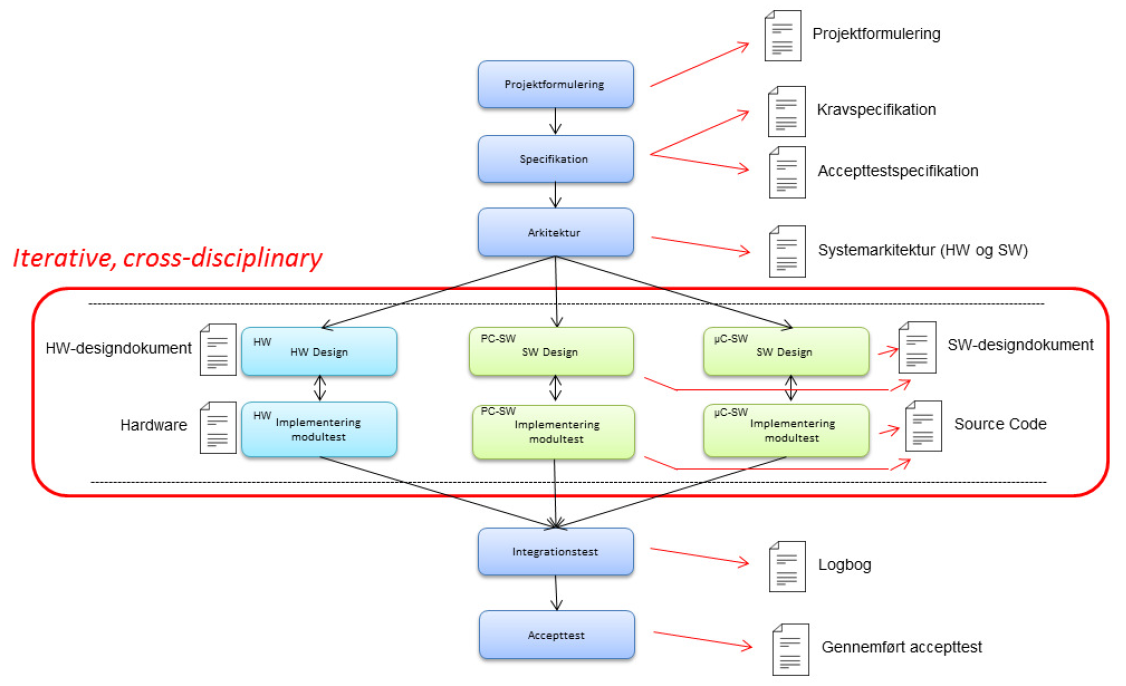
\includegraphics[width=\textwidth]
{Figure/asemodel}}
\caption{ASE-modellen\cite{IngeniorhojskolenAarhusUniversiteta}}
\label{fig:asemodel}
\end{figure}

\begin{figure}[H]
\centering
{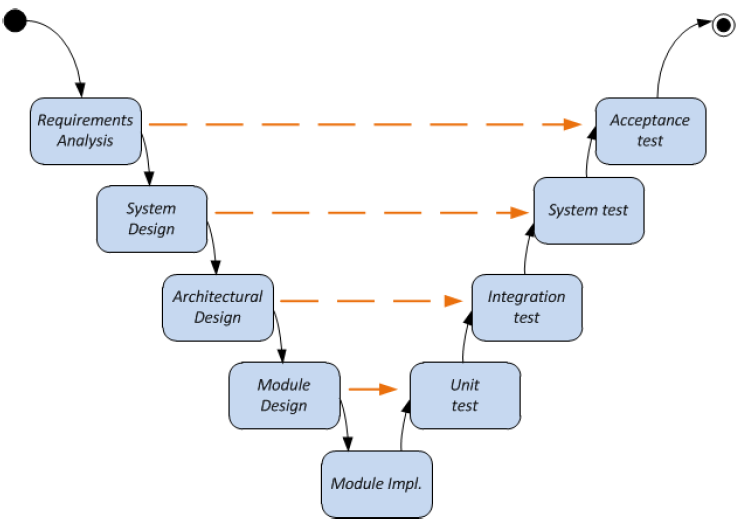
\includegraphics[width=10cm]
{Figure/vmodel}}
\caption{V-modellens udviklingsfaser\cite{IngeniorhojskolenAarhusUniversiteta}}
\label{fig:vmodel}
\end{figure}

Da bachelorprojektet kræver yderligere test og undersøgelser vil denne ASE-model blive modificeret. Der er tilføjet en ekstra fase, analysefasen. Hvilket resulterer i en modificeret ASEmodel
til bachelorprojektet, som kan ses i figur \ref{fig:procesVoresASE}.

\begin{figure}[H]
\centering
{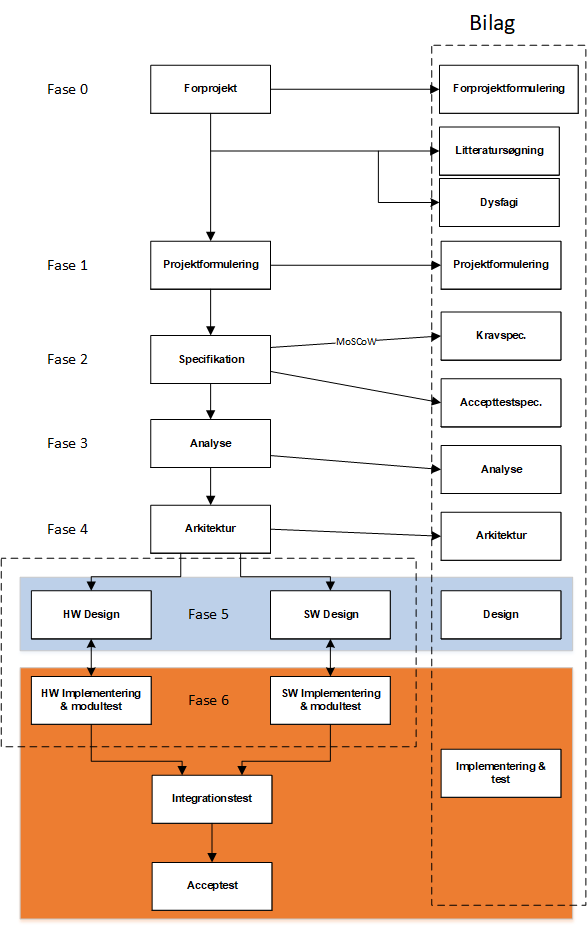
\includegraphics[width=10cm]
{Figure/procesVoresASE}}
\caption{Den modificeret ASE-model.}
\label{fig:procesVoresASE}
\end{figure}

Bachelorprojektets udvikling blev gennemført kan deles op i faserne nul til seks. 

\textbf{Fase 0}\\
Fase nul bestod af et forprojekt, hvor der blev udarbejdet en projektformulering på baggrund af en udleveret projektbeskrivelse og i samarbejde med vejleder. Her blev der udarbejdet udkast til kravspecifikation (MoSCoW analyse) og projektplan. Disse kan ses i \nameref{bilag10}.

\textbf{Fase 1}\\
Fase et bestod i at finde litteratur om emnet dysfagi og udvikling af en måler til at detektere synk. Der blev søgt primærlitteratur ved bl.a. Embase og Pubmed samtidig suppleret med sekundærlitteratur i form af lærebøger fra tidligere semestre. Søgeprotokollen kan ses i \nameref{bilag12}. Dette resulterede i en projektformulering til bachelorprojektet.

\textbf{Fase 2}\\
I fase to blev MoSCoW kravene sat på baggrund af projektformuleringen. Dette resulteret i dokumenterne kravspecifikation og acceptestspecifikation. Kan læses i \nameref{bilag1} og \nameref{bilag2}.

\textbf{Fase 3}\\
Den tredje fase begyndte, vha. af den nye viden og de nye krav, med at udføre analysen. Første del af analysen bestod af at realisere og teste det udleveret kredsløb fra artiklen. Der blev derudover bl.a. undersøgt muligheden for anvendelse af A/D-konverter. Test og undersøgelser blev til dokumentet Analyse, hvilket kan ses i \nameref{bilag3}.

\textbf{Fase 4}\\
Den fjerde fase blev arkitekturen til software og hardware udført, i forlængelse af analysen. Arkitekturen blev dokumenteret ved hjælp af sysML, hvor BDD og IBD diagrammer blev oprettet. Diagrammerne viste hvilke blokke SRM skulle bestå af. Arkitekturen kan læses i \nameref{bilag4}.

\textbf{Fase 5}\\
I femte iterative design fase, blev software og hardware designet. Hardwaren blev dokumenteret med diagrammer, udregninger og stykliste. Software blev dokumenteret med funktions beskrivelser, et sekvensdiagram og et UML-aktivitetsdiagram. Detaljerne kan læses i \nameref{bilag5}.

\textbf{Fase 6}\\
Til sidst i den sjette fase blev software og hardware implementeret, modultestet og samlet til en integrationstest. Til slut blev acceptest udført. Denne fase er samlet i \nameref{bilag6}.

\section{Den gennemførte proces}

Dette afsnit beskriver den ikke-tekniske del af bachelorprojektet.

\textbf{Gruppedannelse}\\
Gruppen består af to sundhedsteknologistuderende, der er dannet udefra en fælles interesse for projektets beskrivelse. Begge medlemmer har, inden valget af projektet, talt sammen om mulige gruppedannelse, hvis der kommer et projekt, hvor begge medlemmer finder det interessant. Det kan siges at gruppen er dannet udefra interessen for projektets indhold og en kendskab til hinanden i forvejen. 

\textbf{Samarbejdsaftale}\\
I dette bachelorprojekt er der genanvendt en samarbejdsaftale fra tidligere semestre med få ændringer. Denne samarbejdsaftale kan læses i \nameref{bilag7}. Her er der beskrevet i bestemte punkter, hvordan gruppen skal arbejde og skal forholde sig under hvert punkt. Den blev godkendt og underskrevet af alle gruppens medlemmer. Udbyttet af at anvende samarbejdsaftalen var positivt for gruppen. Især det benyttet ugeskema gjorde, at man kunne administrere sin tid bedre med fag udover bachelor projektet. 

\textbf{Arbejdsfordeling}\\
Arbejdesbyrden var ligeligt fordelt i mellem gruppemedlemmerne. Hvor den generelle rapportskrivning af afsnit blev tildelt efter hvem der havde tid og hvad der var bedst for bachelorprojektet. Administrationen  af opgaver blev oprettet og styret fra online portalen Pivotal Tracker, som er et Scrum værktøj. Her blev der i fællesskab oprettet opgaver efter pointsystem om hvor vigtig opgaven var. Det var så muligt at tage opgaver og udføre dem, indenfor for et sprint på en uge. Efter en uge ville man kunne få et overblik over afsluttet opgave i det pågældende sprint. En nærmere beskrivelse og brugen af Pivotal Tracker findes i \nameref{bilag16}.

\textbf{Planlægning}\\
I den overordnet planlægning blev der bruget online portalen Teamgantt. Her blev der oprettet en kalender over hele forløbet delt op i forskellige områder fra ASE-modellen. Denne kalender havde hele gruppen adgang til og mulighed for at rette løbende gennem hele projektet. Gruppens brugen af Teamgantt og indstillinger kan læses nærmere i \nameref{bilag16}. For at opreteholde en historik over tidsplanen blev der oprettet en versions historik af tidsplanen, denne kan ses i \nameref{bilag17}.

Det daglige arbejde blev nedskrevet i logbogen ved dagens slutning. Logbogen blev også brugt til at notere beslutninger, ændringer og større arbejde ifm. projektet. For at læse den komplette logbog ses i \nameref{bilag14}.

\textbf{Møder}\\
For at opretholde overblikket og en fast struktur i projektet var der faste møder i gruppen. Hver morgen startet med scrum møde, hvor hvert gruppe medlem fremførte igangværende opgaver og problematikker. Fredagsmødet blev holdt for at kigge tilbage på ugen og det afsluttede sprint. En gang om ugen var der vejledermødet, med en fast dagsorden og de aktuelle emner der blev diskuteret. Alle møder kan læses i \nameref{bilag18}.

\textbf{Projektledelse}\\
I dette bachelor projekt var der valgt ikke at have en projektleder. Der var i stedet valgt en ligefordelt og kollektiv ledelse. Det har gjort at hele gruppen har skulle have overblik i hele projektet. Samtidig har det været med til at alle i gruppen kender målet og retningen og der er tydelige kommunikation og opfølgninger med faste møder og scrum møder hver dag hvor alle deltager i gruppen. Den fælles ledelsesstil har gjort at alle deltagerne er engageret og hele tiden kender målet og er klar til at ændre sådan, at målet opnåes på den bedste mulige måde. Da der er mange praktiske opgaver i bachelorprojekt, er der lavet rollefordeling og ansvarsområder igennem hele projektet. De specifikke roller og ansvarsområder kan ses i \nameref{bilag7}.

\textbf{Projektadministration}\\
Rapporten og bilag er skrevet i tekstsproget Latex. Hvor alle afsnit er delt op i selvstændige .tex filer. Disse afsnit er delt op i en rapport og bilags mappe. Figurer brugt i projektet har også en selvstændig mappe. Møder, referater og logbog er skrevet i Google Docs. Tidsplan og opgaver er oprettet og ligger i selvstændige online værktøjer: Teamgantt og Pivotal Tracker.    

